\documentclass[]{article}

\usepackage[utf8]{inputenc}
\usepackage{amsmath}
\usepackage{amssymb}
\usepackage{amsthm}
\usepackage{amsfonts}
\usepackage{graphicx}
\usepackage{capt-of}
\usepackage{listings}
\usepackage{siunitx}
\usepackage[section]{placeins}
\usepackage{float}



% Oppgavenummerering %
\renewcommand\thesection{Problem \arabic{section}}
\renewcommand\thesubsection{\alph{subsection})}

% Bevis
\newcommand\TombStone{\rule{.5em}{.5em}}
\renewcommand\qedsymbol{\TombStone}
\renewcommand{\proofname}{Bevis.} % Norske bevis

\title{TTK4215 – Assignment 8}
\author{Sigurd Totland | MTTK}

\begin{document}
\maketitle

\section{I\&S 6.1}
We have the system
\begin{equation}\begin{aligned}
y = \frac{b}{s-1}u
\end{aligned}\end{equation}
that we wish to control using direct model reference adaptive control using the model
\begin{equation}\begin{aligned}
y_m = \frac{2}{s+2}r.
\end{aligned}\end{equation}
This design corresponds to the one presented in I\&S example 6.2.2, with
\begin{equation}\begin{aligned}
x=y, \quad a = 1, \quad a_m = 2, \quad b_m = 2,
\end{aligned}\end{equation}
and $b > 0$ unknown, but with known sign. The signals $y$, $y_m$ and the reference $r$ are known signals. Since this is direct control, we wish to estimate the controller parameters directly. We define
\begin{equation}\begin{aligned}
k^* = \frac{a_m + a}{b} = \frac{3}{b}, \quad \text{and} \quad
l^* = \frac{b_m}{b} = \frac{2}{b}
\end{aligned}\end{equation}
and wish to use the control law
\begin{equation}\begin{aligned}
u = -k^*y + l^* r.
\end{aligned}\end{equation}
We then see the need for the requirement $b > 0$, as we cannot allow $b$ to cross zero and cause the controller parameters to blow up. However, since $k^*$ and $l^*$ are unknown parameters, we cannot use this controller, so we instead define the control law
\begin{equation}\begin{aligned}
u = -k(t)y + l(t) r,
\end{aligned}\end{equation}
where $k$ and $l$ are corresponding estimates. We define the tracking error
\begin{equation}\begin{aligned}
e = y - y_m,
\end{aligned}\end{equation}
as well as the estimation error
\begin{equation}\begin{aligned}
\epsilon_1 = e - \hat e,
\end{aligned}\end{equation}
but since we can measure $y$, $\hat e = 0$ and so $\epsilon_1 = e$. We then get the adaptive laws according to (6.2.29), i.e.
\begin{equation}\begin{aligned}
\dot k &= \gamma_1 \epsilon_1 y sgn(b) = \gamma_1 \epsilon_1 y,\\
\dot l &= \gamma_2 \epsilon_1 r sgn(b) = \gamma_2 \epsilon_1 r.
\end{aligned}\end{equation}
We can write up a block diagram for this like shown in figure \ref{fig:mrac1} below.
\begin{figure}[H]
\centering
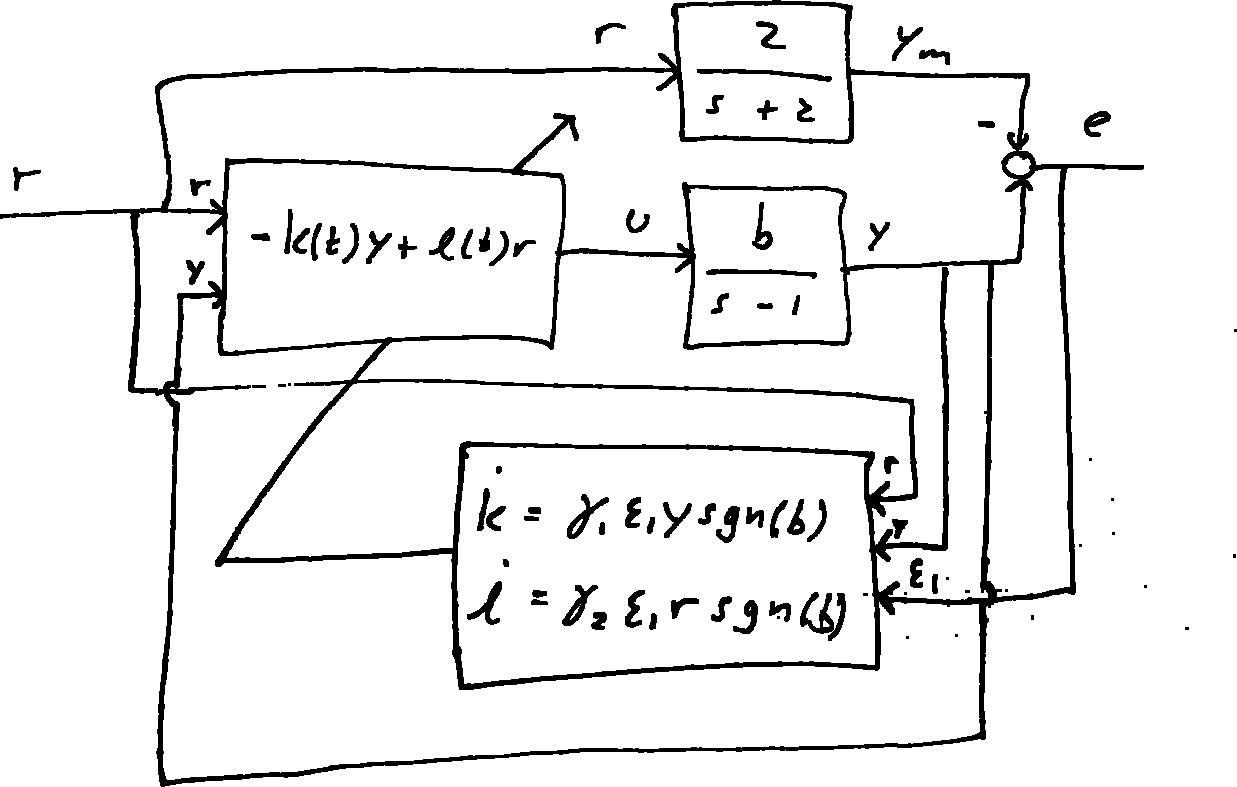
\includegraphics[width=0.8\textwidth]{mrac1}
\caption{MRAC block diagram}
\label{fig:mrac1}
\end{figure}

\section{I\&S 6.2}
\subsection{}
Given the system
\begin{equation}\begin{aligned}
V = \frac{b}{s+a}\theta + d
\label{eq:sys}
\end{aligned}\end{equation}
where $d$ is constant a disturbance, and a reference model
\begin{equation}\begin{aligned}
V_m = \frac{0.5}{s = 0.5}V_s
\end{aligned}\end{equation}
i.e., unknown parameters $b>0$, $a$ and $d$ and known model parameters $a_m = 0.5$ and $b_m = 0.5$.
In the first case, we assume the unknown parameters are actually known. We rewrite the system to
\begin{equation}\begin{aligned}
V(s+a) = b \theta + ds + da
\end{aligned}\end{equation}
and note that since $d$ is a constant disturbance, $ds = 0$, meaning we get
\begin{equation}\begin{aligned}
\label{eq:datboi}
Vs = -aV + b \theta + da.
\end{aligned}\end{equation}
With MRC, we want
\begin{equation}\begin{aligned}
V = V_m.
\end{aligned}\end{equation}
We want a controller with a feed forward term, a feedback term and a constant term to combat the constant disturbance, i.e. we want
\begin{equation}\begin{aligned}
\theta = k^* V - l^*V_s - m^*
\end{aligned}\end{equation}
where $k^*$, $l^*$ and $m^*$ are constants. We insert this into \eqref{eq:datboi} and obtain
\begin{equation}\begin{aligned}
Vs = -aV + b(k^* - l^* - m^*) + da
\end{aligned}\end{equation}
$sd=0$ since the disturbance is constant. We then get
\begin{equation}\begin{aligned}
sV &= -a(a - bk^*)V + bl^* V_s - bm^* + ad \\
&= -(a - bk^*) V + \frac{bl^*}{b_m}(V_ms+a_mV_m) - bm^* + ad
\end{aligned}\end{equation}
We rewrite this to
\begin{equation}\begin{aligned}
sV + (a-bk^*)V = \frac{bl^*}{b_m}V_ms + \frac{bl^*a_m}{b_m}V_m - b_m m^* + ad.
\end{aligned}\end{equation}
Now, to make $V=V_m$ as well as $sV = sV_m$, we must require
\begin{equation}\begin{aligned}
m^* = \frac{ad}{b}, \quad l^* = \frac{b_m}{b}
\end{aligned}\end{equation}
and with
\begin{equation}\begin{aligned}
a - bk^* = \frac{bl^* a_m}{b_m} \implies bk^* = a - \frac{bl^* a_m}{b_m} = a-a_m
\end{aligned}\end{equation}
we obtain
\begin{equation}\begin{aligned}
k^* = \frac{a-a_m}{b}.
\end{aligned}\end{equation}
Of course, we must know the sign of $b > 0$ for these parameters not to go to infinity.
\end{document}

